\chapter{Usabilità sul Campo}
\label{cap:usabilita}
\section{Raccolta feedback}

Uno dei pilastri della nostra strategia di usabilità per DietiEstates25 è stato l'ascolto attivo degli 
utenti. Quando sono emersi dubbi su come strutturare al meglio la fase di registrazione, invece di 
affidarci solo all'intuizione, abbiamo mostrato diverse bozze ai potenziali utilizzatori. Le loro 
opinioni ci hanno guidato nella scelta della soluzione finale, assicurando che il sistema fosse semplice 
e chiaro sin dal primo accesso.

\vspace{0.3cm}

Abbiamo esteso questa strategia di validazione empirica alla definizione della \textbf{Dashboard principale 
(Home)}.

\begin{figure}[H]
    \centering
    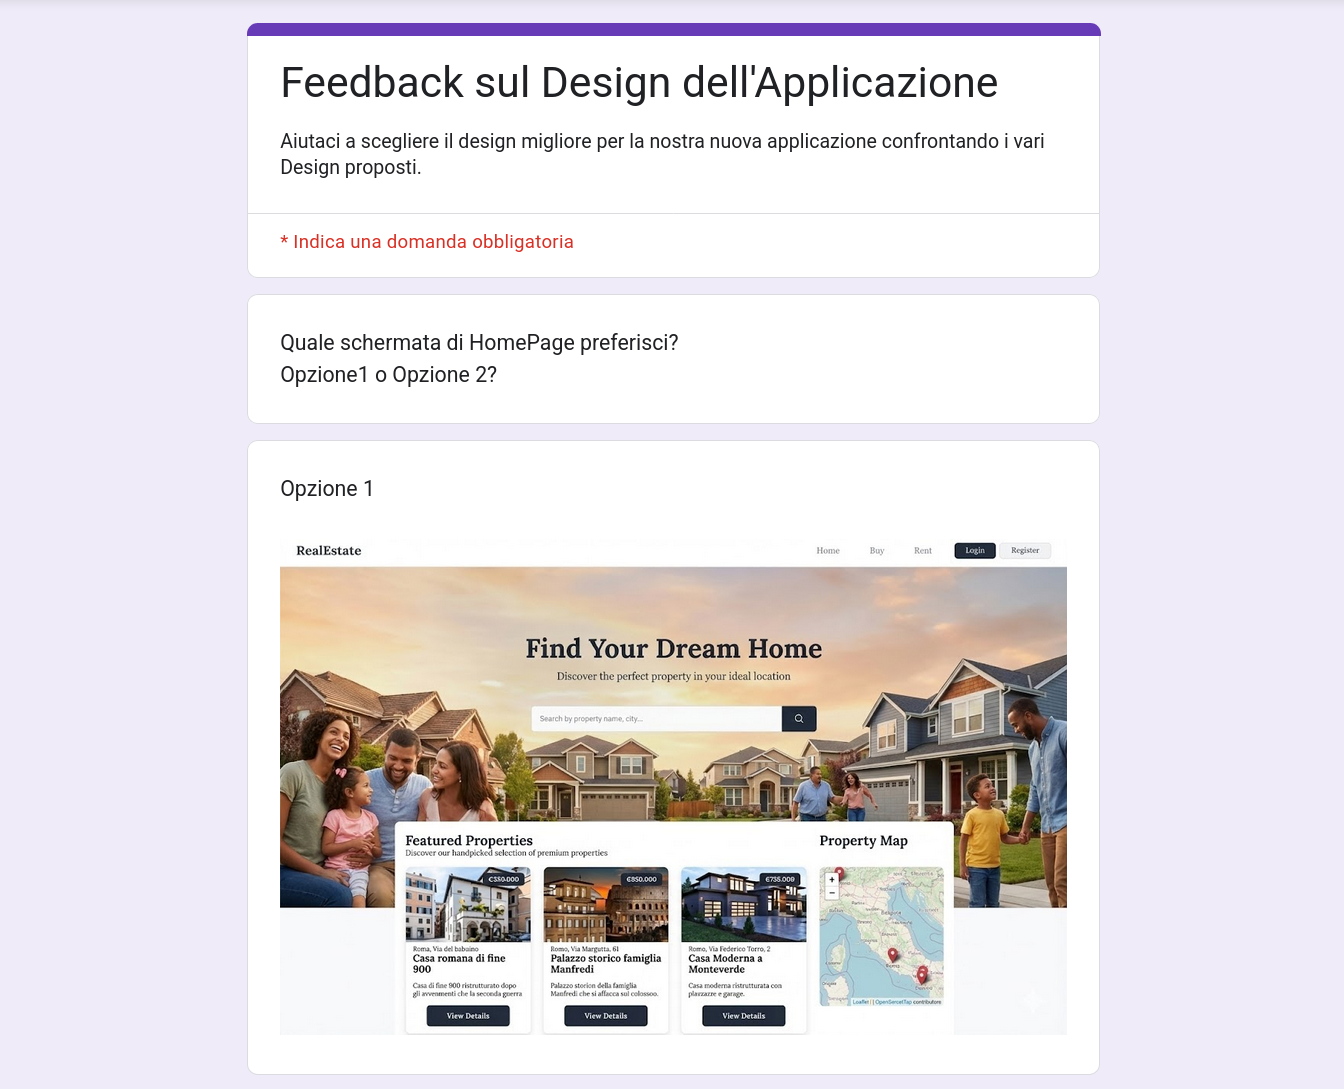
\includegraphics[width=0.8\textwidth]{images/Feedback1.png}
    \caption{Opzione 1 - Dashboard Home}
    \label{fig:Feedback1}
\end{figure}

\begin{figure}[H]
    \centering
    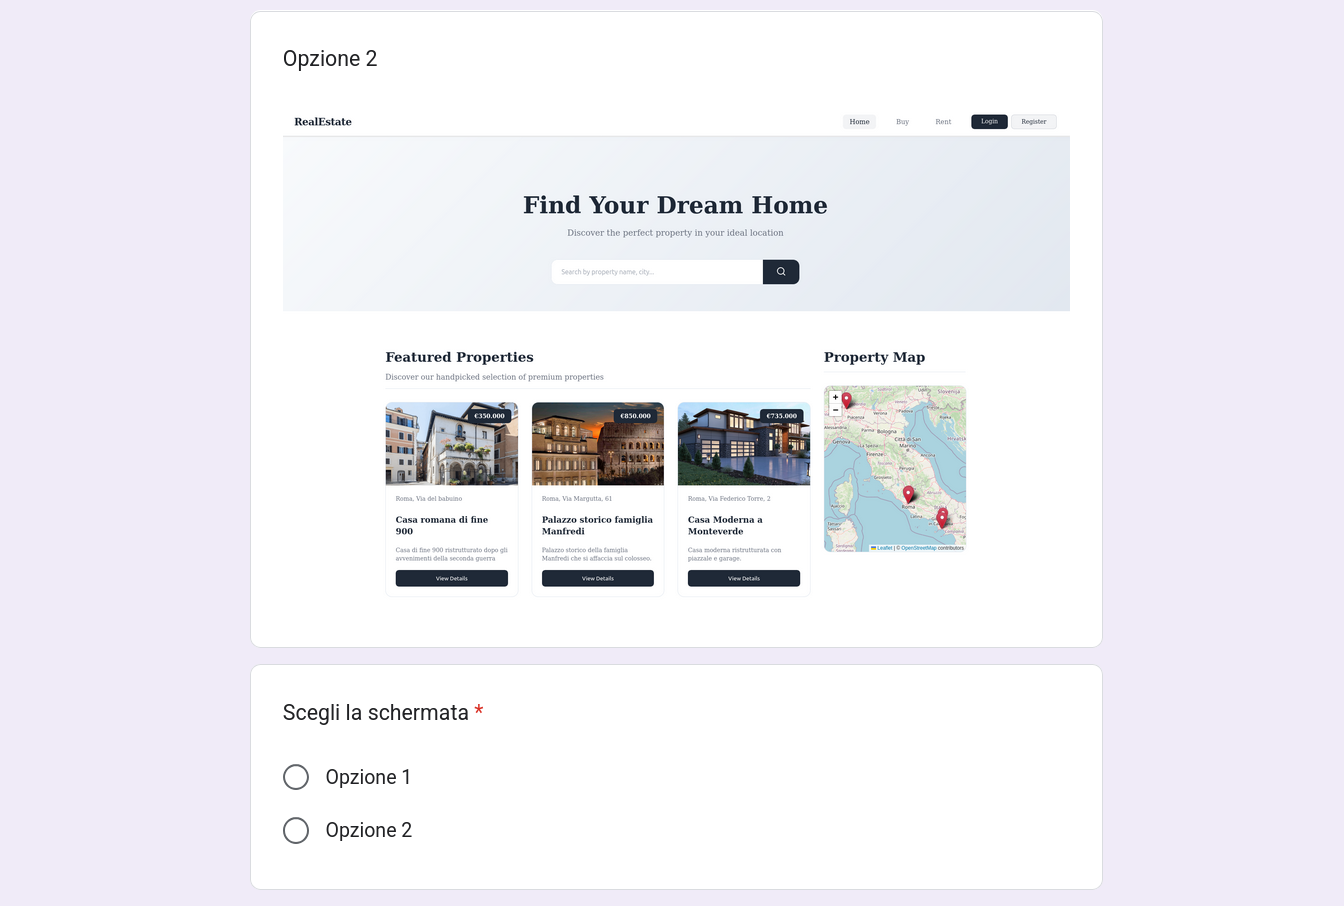
\includegraphics[width=0.8\textwidth]{images/Feedback2.png}
    \caption{Opzione 2 - Dashboard Home}
    \label{fig:Feedback2}
\end{figure}

Sottoponendo al campione di utenti diverse filosofie di interfaccia, è emersa una preferenza quasi 
unanime per l'\textbf{Opzione 2}, caratterizzata da un design moderno e arioso (whitespace-oriented). 
I feedback hanno confermato che, in un portale immobiliare, l'utente non cerca un sovraccarico di 
informazioni immediate, ma una \textbf{gerarchia visiva rigorosa} che trasmetta professionalità.

\vspace{0.3cm}

\begin{figure}[H]
    \centering
    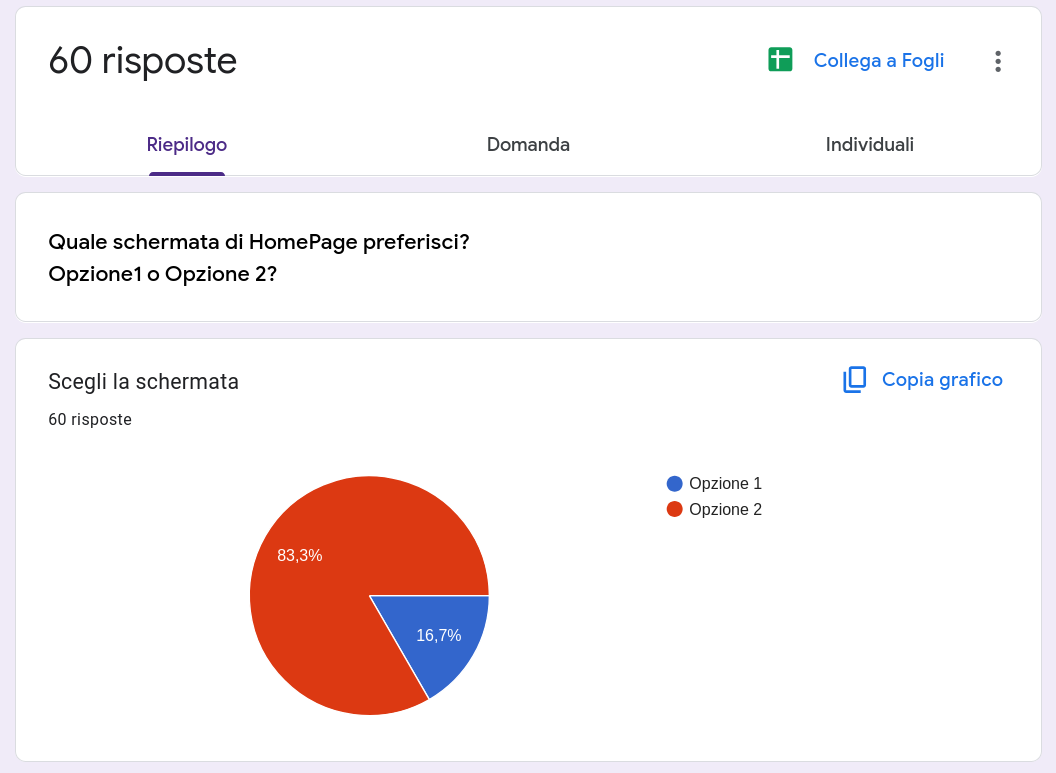
\includegraphics[width=0.8\textwidth]{images/RisposteFeedback1.png}
    \caption{Risultati del Feedback sulla Dashboard Home}
    \label{fig:RisposteFeedback1}
\end{figure}

\vspace{0.3cm}

La soluzione adottata risponde dunque a un preciso desiderio di chiarezza: ogni elemento — dalle card 
degli immobili ai filtri di ricerca — gode del giusto spazio per essere fruito senza sforzo cognitivo, 
facilitando l'orientamento immediato.

\vspace{0.3cm}

La stessa metodologia ha guidato la progettazione delle schermate di \textbf{Autenticazione e Registrazione}.

\begin{figure}[H]
    \centering
    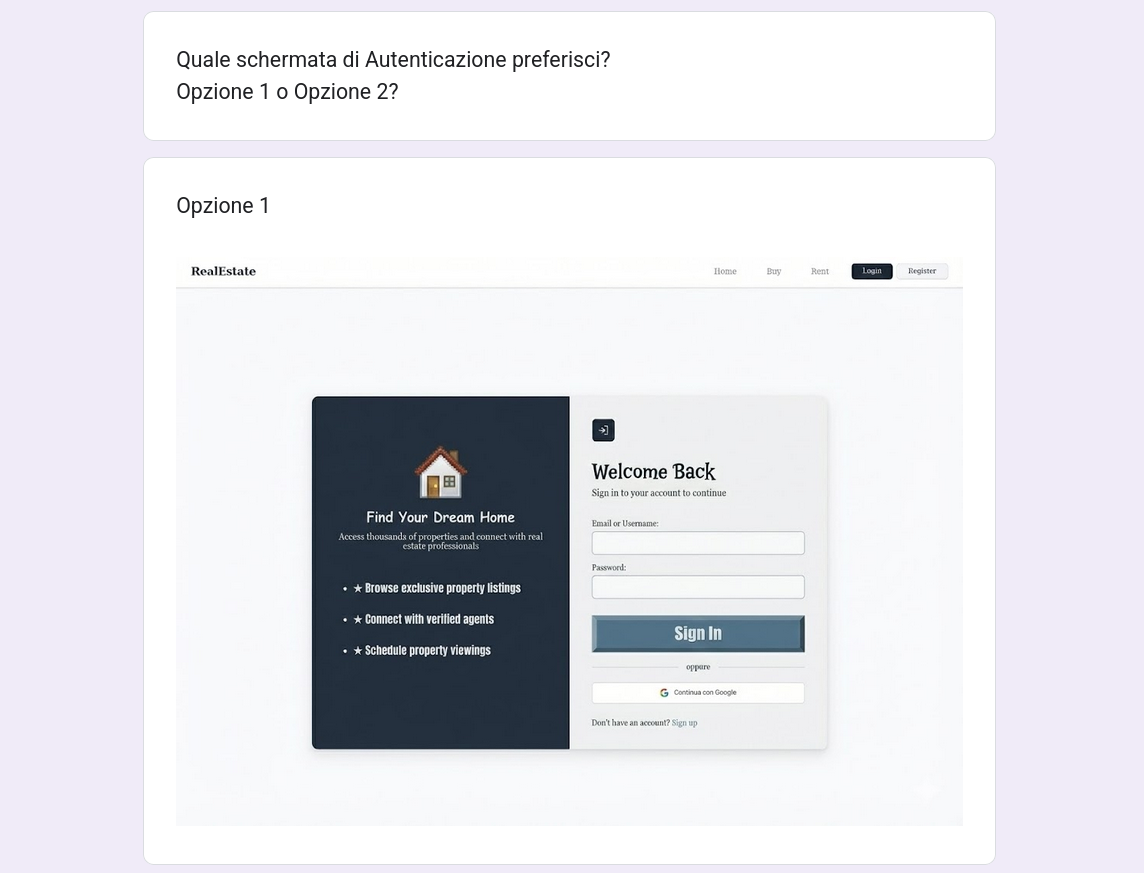
\includegraphics[width=0.8\textwidth]{images/FeedbackLogin1.png}
    \caption{Opzione 1 - Interfaccia Login/Registrazione}
    \label{fig:FeedbackLogin1}
\end{figure}

\begin{figure}[H]
    \centering
    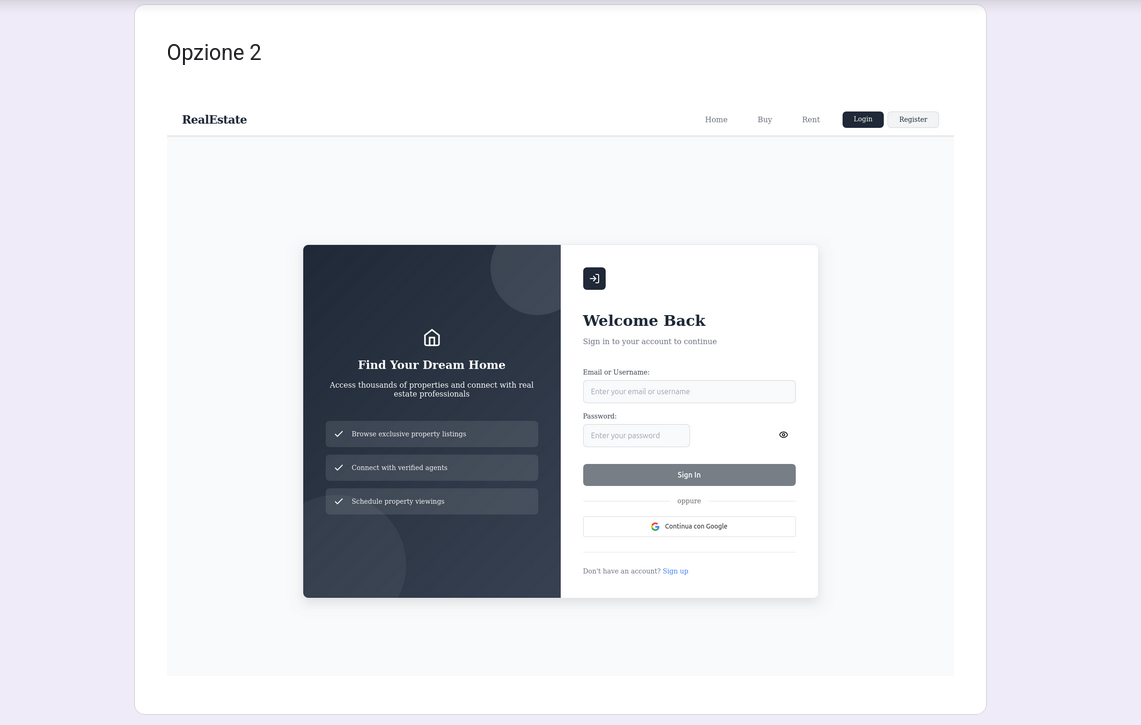
\includegraphics[width=0.8\textwidth]{images/FeedbackLogin2.png}
    \caption{Opzione 2 - Interfaccia Login/Registrazione}
    \label{fig:FeedbackLogin2}
\end{figure}

\begin{figure}[H]
    \centering
    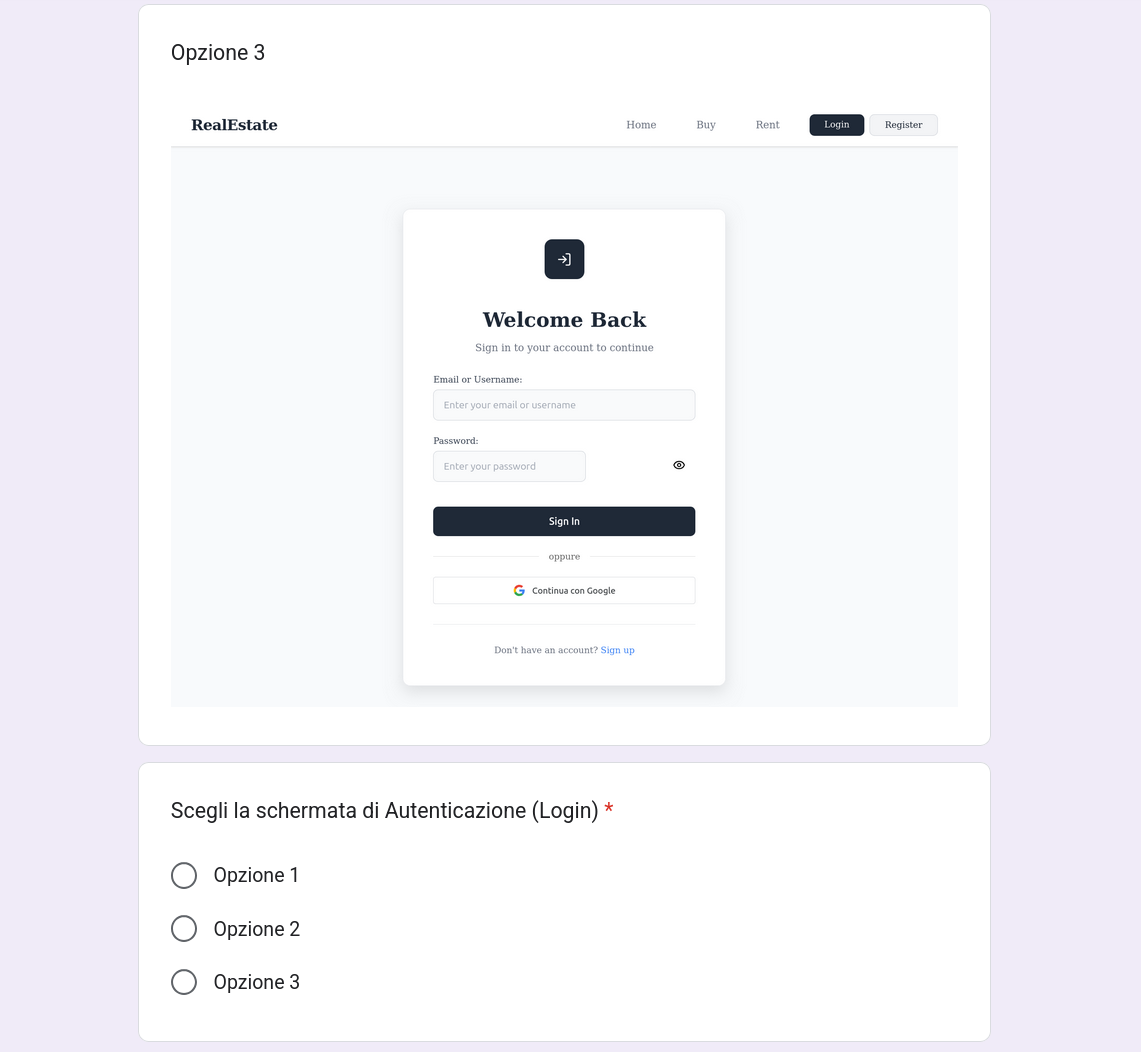
\includegraphics[width=0.8\textwidth]{images/FeedbackLogin3.png}
    \caption{Opzione 3 - Interfaccia Login/Registrazione}
    \label{fig:FeedbackLogin3}
\end{figure}

Anche in questo frangente, gli utenti hanno premiato l'Opzione 2, lodandone la capacità di bilanciare 
funzionalità ed emozione. L'analisi dei feedback ha rivelato che il \textbf{layout Split-Screen (schermo 
diviso)} è stato percepito come il più rassicurante: da un lato, l'area funzionale su sfondo chiaro 
offre la massima leggibilità per l'inserimento dati; dall'altro, la sezione dedicata al branding — 
con messaggi come "Join Our Community" — lavora sull'aspetto psicologico. Questo approccio non solo 
rende l'interfaccia pulita, ma riduce la freddezza burocratica del modulo, facendo sentire l'utente 
parte di una comunità esclusiva fin dal primo accesso.

\vspace{0.3cm}

\begin{figure}[H]
    \centering
    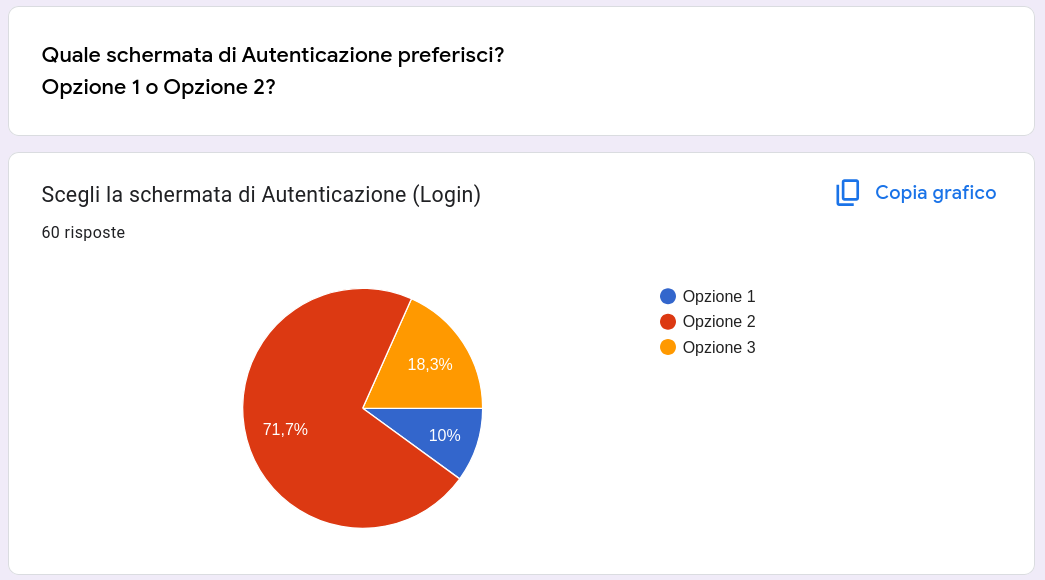
\includegraphics[width=0.8\textwidth]{images/RisposteFeedback2.png}
    \caption{Risultati del Feedback sulle Interfacce di Login/Registrazione}
    \label{fig:RisposteFeedback2}
\end{figure}